\section{The ladder}\label{dc:sec:ladder}

Restrict the support of $h$. For $a>0$ and $\varepsilon\ge0$ let
\begin{multline*}
\lambda_{\min}\big(\tfrac12+\varepsilon,a\big)=\inf\Big\{\frac{Q_\varepsilon(h)}{\|h\|_2^2}:h\text{ bounded, real, of bounded variation,}\\ \text{supported in }[-a,a],\ h\ne0\Big\}.
\end{multline*}
This is the least eigenvalue $\lambda_{\min}(\alpha,a)$, $\alpha=\frac12+\varepsilon$, of Chapter~\ref{chap:yoshida}, with the same normalisation. The function $e^{-\varepsilon|x|}(h*\tilde h)$ is supported in $[-2a,2a]$, so $Q_\varepsilon$ involves only the prime powers $n\le e^{2a}$: each $\lambda_{\min}(\frac12+\varepsilon,a)$ is the bottom of the spectrum of an explicit form. RH is $\lambda_{\min}(\frac12,a)\ge0$ for every $a$. Yoshida~\cite[Theorem 1]{Yoshida92} proved positivity of Weil's form for $a\le\frac12\log2$, the range in which no prime enters, Bombieri~\cite{Bombieri} treated other test functions of small support, and Connes and Consani reproved Yoshida's range from the semilocal trace formula~\cite{ConnesConsani21}. Zhu certifies the lower bound $8.9\times10^{-18}$ for $\lambda_{\min}(\frac12,a)$ at $a=0.8$ (Corollary 6.3 of \cite{Zhu26}), and reports an empirical law for the decay of $\lambda_{\min}(\frac12,a)$~\cite{Zhu26} (Chapter~\ref{chap:zhu}), and Connes, Consani and Moscovici find that the Fourier transform of the lowest eigenvector of a truncated form reproduces the low zeros to high accuracy~\cite{CCM25}. The last two papers are cited as preprints.
% CHECK: the pinpoint Theorem 1 of Yoshida92 for the window (1/2) log 2 is unverified; Zhu's preprint (misc/reviews/nick-zhu/zhu-arxiv/zhu.txt, abstract and Section 1) attributes to Yoshida positivity for 2L <= log 2 and to Connes and Consani a second proof of this range, which supports the text
% CHECK: the statement attributed to Connes, Consani and Moscovici (the Fourier transform of the lowest eigenvector of a truncated Weil form reproduces the low zeros to high accuracy) rests on the first author's check of the abstract and Corollary 3.8 of arXiv:2511.22755 and is not verified by the citation verifier

\begin{theorem}[The ladder at depth $\varepsilon>0$]\label{dc:thm:ladder}
Let $\varepsilon>0$ be to the right of the zeros, and suppose that $v_{1/2+\varepsilon}(\theta)>v_{1/2+\varepsilon}(0)$ for $\theta\ne0$, with $v_{1/2+\varepsilon}''(0)>0$ and $\liminf_{|\theta|\to\infty}v_{1/2+\varepsilon}(\theta)>v_{1/2+\varepsilon}(0)$.
\begin{enumerate}
\item[(a)] $\lambda_{\min}(\frac12+\varepsilon,a)$ is nonincreasing in $a$, and $\lambda_{\min}(\frac12+\varepsilon,a)\ge2b_{1/2+\varepsilon}>0$ for every $a$.
\item[(b)] $\lambda_{\min}(\frac12+\varepsilon,a)\to2b_{1/2+\varepsilon}$ as $a\to\infty$, and there are constants $c,a_0>0$ with
\[
\frac{c}{a^2}\le\lambda_{\min}\big(\tfrac12+\varepsilon,a\big)-2b_{1/2+\varepsilon}\le\frac{\pi^2v_{1/2+\varepsilon}''(0)/4+o(1)}{a^2}\qquad(a\ge a_0).
\]
\item[(c)] At $\varepsilon=0$, with none of the hypotheses above, under RH, $\lambda_{\min}(\frac12,a)\ge0$ and $\lambda_{\min}(\frac12,a)=O(a^{-N})$ for every $N$, so $\lambda_{\min}(\frac12,a)\to0$; if RH fails, $\lambda_{\min}(\frac12,a)<0$ for all large $a$.
\end{enumerate}
\end{theorem}

\begin{proof}
(a) is Theorem~\ref{yo:thm:coercive}(i) of Chapter~\ref{chap:yoshida} at $\alpha=\frac12+\varepsilon$, whose $m_\alpha=\inf_\theta v_\alpha(\theta)$ is $b_\alpha$ here, the minimum being at the origin; and $b_{1/2+\varepsilon}=\sum_\rho\re(\frac12+\varepsilon-\rho)^{-1}>0$ because every term is positive. We use the first step of that proof: by~\eqref{dc:eq:Qw} and Parseval, $\|\hat h\|_2^2=2\pi\|h\|_2^2$, so $Q_\varepsilon(h)/\|h\|_2^2=2\langle v_{1/2+\varepsilon}\rangle_h$, the average of $v_{1/2+\varepsilon}$ against the probability density $|\hat h|^2/\|\hat h\|_2^2$, which is at least $2\min v_{1/2+\varepsilon}=2b_{1/2+\varepsilon}$.

(b) Write $v=v_{1/2+\varepsilon}$. Upper bound: take $h(u)=\cos(\pi u/2a)$ on $[-a,a]$. Then $\langle\theta^2\rangle_h=\|h'\|_2^2/\|h\|_2^2=\pi^2/4a^2$, and the normalised density satisfies $|\hat h(\theta)|^2/\|\hat h\|_2^2=O(a^{-3}\theta^{-4})$ for $|\theta|\ge1/a$. Write $v(\theta)=v(0)+\frac12v''(0)\theta^2+R(\theta)$, with $|R(\theta)|\le C\theta^4$ for $|\theta|\le\eta$ and $|R(\theta)|\le C\theta^2\log(2+|\theta|)$ for all $\theta$. Splitting at $|\theta|=\eta$ gives $\langle R\rangle_h=O(\eta a^{-3})+O(a^{-3}\eta^{-1})$, and with $\eta=a^{-1/2}$ this is $o(a^{-2})$. Hence $\lambda_{\min}(\frac12+\varepsilon,a)\le2v(0)+v''(0)\pi^2/4a^2+o(a^{-2})$. Lower bound: by the hypotheses there is $c_1>0$ with $v(\theta)-v(0)\ge c_1\min(\theta^2,1)$. For $h$ supported in $[-a,a]$ the fraction of $\|\hat h\|_2^2$ carried by $|\theta|\le\kappa/a$ is at most the largest eigenvalue $\ell_0(\kappa)$ of the time and band limiting operator with product $\kappa$, which is less than $1$ for every finite $\kappa$ and tends to $0$ with $\kappa$~\cite{SlepianPollak61}. So $\langle\min(\theta^2,1)\rangle_h\ge(\kappa/a)^2(1-\ell_0(\kappa))$ once $\kappa\le a$, which is the lower bound with $c=2c_1\kappa^2(1-\ell_0(\kappa))$. Convergence $\lambda_{\min}(\frac12+\varepsilon,a)\to2b_{1/2+\varepsilon}$ follows from the two bounds.

(c) Under RH, $Q_0(h)=\sum_\gamma|\hat h(\gamma)|^2\ge0$ by Theorem~\ref{dc:thm:weil}. Fix a real $h_1\in C_c^\infty[-1,1]$, $h_1\ne0$, and put $h_a(u)=h_1(u/a)$. Then $\hat h_a(\theta)=a\hat h_1(a\theta)$ with $|\hat h_1(t)|\le C_N|t|^{-N}$, so $Q_0(h_a)/\|h_a\|_2^2\le C_N'a^{1-2N}\sum_\gamma\gamma^{-2N}$, every $|\gamma|$ being larger than $14$. If RH fails, Weil's criterion gives $h\in C_c^\infty$, which may be taken real, with $Q_0(h)<0$; it is supported in some $[-a_0,a_0]$, and by monotonicity $\lambda_{\min}(\frac12,a)\le\lambda_{\min}(\frac12,a_0)<0$ for $a\ge a_0$.
\end{proof}

At $\varepsilon=\frac12$ the hypotheses of the theorem hold with no assumption on the zeros: the level is to the right of the zeros because $\zeta$ has no zeros on $\re s=1$, and Proposition~\ref{bp:prop:v1min} gives the minimum at the origin, with $v_1''(0)>0$, and in its proof $v_1>0.05>b_1$ for $|\theta|\ge2000$, which is the third condition. For $0<\varepsilon<\frac12$ the level is to the right of the zeros exactly when the closed half plane $\re s\ge\frac12+\varepsilon$ is free of zeros, which the announced half plane gives only for $\varepsilon>\frac38$; the minimum at the origin is certified for $0<|\theta|\le H_0-\frac{1+\sqrt2}2$, $H_0=3\times10^{12}$, by Theorem~\ref{thm:dbeta:minall}(ii) (Table~\ref{tab:dbeta:minall}), and its holding on every line with $\frac12<\alpha<1$ jointly is equivalent to RH (part (vi) there). The third condition is not known for $0<\varepsilon<\frac12$ without RH; under RH it holds, because $v_{1/2+\varepsilon}$ is then a sum of Poisson kernels of the zeros and tends to infinity.

\begin{remark}\label{dc:cor:half}
At $\varepsilon=\frac12$ the hypotheses of Theorem~\ref{dc:thm:ladder}(a) and (b) hold, as just said, and $2b_1=2\frac{\xi'}{\xi}(1)=2\big(1+\frac{\gamma_E}2-\frac12\log4\pi\big)=2+\gamma_E-\log4\pi=0.0461914\ldots$. So for every $a>0$ and every bounded real $h$ of bounded variation supported in $[-a,a]$,
\[
Q_{1/2}(h)\ \ge\ \big(2+\gamma_E-\log4\pi\big)\,\|h\|_2^2=0.0461914\ldots\,\|h\|_2^2,
\]
and by~\eqref{dc:eq:Qw} this is Proposition~\ref{bp:prop:v1min} read through Plancherel, and Theorem~\ref{yo:thm:coercive}(i) at $\alpha=1$, which is Corollary~\ref{yo:cor:half} of Chapter~\ref{chap:yoshida}; what the ladder adds is the rate in $a$ of Theorem~\ref{dc:thm:ladder}(b).
\end{remark}

\subsection{Numerical results}\label{dc:sec:numerics}

We computed $\lambda_{\min}(\frac12+\varepsilon,a)$ variationally, with $h$ in the span of the first $M$ Legendre polynomials $q_0,\dots,q_{M-1}$ on $[-a,a]$, normalised in $L^2$: the correlations $q_j*\tilde q_k$ by Gauss Legendre quadrature, which is exact for polynomials; the archimedean and pole integrals by Gauss Legendre quadrature on $[0,2a]$, plus the exact tail of the $g(0)$ term; and the primes exactly. The script \texttt{dc\_ladder.py} (\texttt{code/\allowbreak README.md}) repeats this for $M=24$ to $128$ and computes the same eigenvalue on a second basis, the normalised Fourier modes $e^{i\pi nu/a}$, $|n|\le N$, for $N=24$ to $1536$, from the matrices of the module \texttt{yo\_matrix.py} of Chapter~\ref{chap:yoshida}. Every computed eigenvalue is an upper bound for $\lambda_{\min}$, since a finite basis is a variational class, and needs no hypothesis on the zeros, because $Q_\varepsilon$ is an explicit finite form; the hypotheses of Theorem~\ref{dc:thm:ladder} enter only in what the numbers are compared with. Rounding is not the limit: double precision agrees with thirty digit arithmetic to $1.4\times10^{-14}$ at most, and $1.5$ times the quadrature nodes changes the eigenvalue by at most $2\times10^{-15}$. The limit is the size of the basis.

Between $M=24$ and $M=32$ the Legendre bounds change by at most $2.6\times10^{-6}$, but they are not converged at that level: for $\varepsilon>0$ the $M=32$ values lie above the converged values defined next by $0.6\times10^{-7}$ to $1.8\times10^{-6}$, so the change between two sizes understates the error. The Fourier sections are nested, and their eigenvalues converge like a power, $\lambda_N-\lambda_\infty\propto N^{-p}$ with $p$ between $1.18$ and $1.69$ over the whole grid. The \emph{converged value} is the power law extrapolation from the three largest sizes $N=384$, $768$, $1536$, and its uncertainty is the shift of that value when the largest size is dropped (sizes $192$, $384$, $768$): at most $2.7\times10^{-8}$ at $a=0.25$, $3.0\times10^{-9}$ at $a=0.5$ and $1.7\times10^{-9}$ for $a\ge0.75$. This is an error estimate and not a bound. Two checks support it. The Legendre bound with $M=128$ lies above the converged value in all $40$ entries with $\varepsilon>0$, by $1.8\times10^{-8}$ to $1.5\times10^{-7}$, as an upper bound must. And the converged values of Table~\ref{yo:tab:lam} of Chapter~\ref{chap:yoshida}, obtained there by Richardson extrapolation of the sizes $N=96$, $192$, $384$, agree with the values computed here for the same cells to $2.0\times10^{-8}$ at most over its twenty entries with $\alpha>\frac12$ and to $4.1\times10^{-9}$ for $a\ge0.8$.

Table~\ref{dc:tab:ladder} shows the converged values for $\varepsilon>0$ and, at $\varepsilon=0$, for $a=0.25$ and $0.5$, and Table~\ref{dc:tab:zero} the rung at $\varepsilon=0$ for $0.25\le a\le0.5$. Table~\ref{yo:tab:lam} of Chapter~\ref{chap:yoshida} and Table~\ref{zh:tab:hp} of Chapter~\ref{chap:zhu} list eigenvalues of the same kind for other windows and levels; the level $0.375$ of Table~\ref{dc:tab:ladder} is that of the announced half plane. Figure~\ref{dc:fig:ladder} plots the eigenvalue on a logarithmic scale.

\begin{table}[ht]
\centering\small
\setlength{\tabcolsep}{4pt}
\begin{tabular}{@{}rcccccc@{}}
\toprule
$a$ & $\varepsilon=0.5$ & $0.375$ & $0.2$ & $0.1$ & $0.05$ & $0$\\
\midrule
$0.25$ & $0.0894856$ & $0.0756372$ & $0.0560458$ & $0.0447429$ & $0.0390618$ & $0.0333609$\\
$0.5$ & $0.0495266$ & $0.0372606$ & $0.0200130$ & $0.0100860$ & $0.0050779$ & $9.33\times10^{-7}$\\
$0.75$ & $0.0474318$ & $0.0355980$ & $0.0190070$ & $0.0095123$ & $0.0047593$ & \\
$1$ & $0.0468396$ & $0.0351417$ & $0.0187506$ & $0.0093779$ & $0.0046899$ & \\
$1.5$ & $0.0464620$ & $0.0348541$ & $0.0185931$ & $0.0092974$ & $0.0046489$ & \\
$2$ & $0.0463394$ & $0.0347613$ & $0.0185428$ & $0.0092720$ & $0.0046361$ & \\
$3$ & $0.0462555$ & $0.0346979$ & $0.0185087$ & $0.0092548$ & $0.0046275$ & \\
$4$ & $0.0462270$ & $0.0346764$ & $0.0184971$ & $0.0092490$ & $0.0046246$ & \\
\midrule
$2b_{1/2+\varepsilon}$ & $0.0461914$ & $0.0346497$ & $0.0184828$ & $0.0092418$ & $0.0046210$ & $0$\\
\bottomrule
\end{tabular}
\caption{The ladder $\lambda_{\min}(\frac12+\varepsilon,a)$, converged values: the limit of the variational upper bounds on the Fourier modes $e^{i\pi nu/a}$, $|n|\le N$, by power law extrapolation from $N=384$, $768$, $1536$ (\texttt{code/dc\_ladder.py}, parts \texttt{grid} for $\varepsilon>0$ and \texttt{y0} for $\varepsilon=0$, \texttt{data/dc\_ladder.json}). The uncertainty of an entry is the one defined in the text; it is an error estimate and not a bound. The last row is the limit $2b_{1/2+\varepsilon}=2\,\xi'/\xi(\frac12+\varepsilon)$ of Theorem~\ref{dc:thm:ladder} where its hypotheses hold (for $\varepsilon<\frac12$ they are conditional, and at $\varepsilon=0$ the limit is $0$ under RH), computed by \texttt{code/dc\_weil.py}, part W2 (\texttt{data/dc\_weil.json}). At $\varepsilon=0$ the entries for $a\ge0.75$ are omitted: in double precision they are below the rounding level of about $10^{-13}$, and the upper bounds from extended precision are given in the text.}
\label{dc:tab:ladder}
\end{table}

\begin{table}[ht]
\centering\small
\begin{tabular}{@{}cccc@{}}
\toprule
$a$ & $M=32$ & converged & uncertainty\\
\midrule
$0.25$ & $3.3363\times10^{-2}$ & $3.3361\times10^{-2}$ & $2.7\times10^{-8}$\\
$0.3$ & $7.5722\times10^{-3}$ & $7.5715\times10^{-3}$ & $1.4\times10^{-8}$\\
$\frac12\log2$ & $1.3294\times10^{-3}$ & $1.3293\times10^{-3}$ & $3.4\times10^{-9}$\\
$0.35$ & $1.1938\times10^{-3}$ & $1.1935\times10^{-3}$ & $1.3\times10^{-9}$\\
$0.4$ & $1.8173\times10^{-4}$ & $1.8126\times10^{-4}$ & $1.1\times10^{-9}$\\
$0.45$ & $1.6232\times10^{-5}$ & $1.6149\times10^{-5}$ & $1.7\times10^{-10}$\\
$0.5$ & $9.4039\times10^{-7}$ & $9.3317\times10^{-7}$ & $1.4\times10^{-11}$\\
\bottomrule
\end{tabular}
\caption{The rung at $\varepsilon=0$ for $a\le0.5$: the Legendre bound with $M=32$, the converged value (Fourier modes to $1536$, power law extrapolation) and its uncertainty, the shift of the extrapolation when $N=1536$ is dropped, an error estimate and not a bound. At $a=\frac12\log2=0.3466$, the largest window in which no prime enters, the value is $1.3293\times10^{-3}$. Script \texttt{code/dc\_ladder.py}, part \texttt{y0}, data \texttt{data/dc\_ladder.json}.}
\label{dc:tab:zero}
\end{table}

For every level in Table~\ref{dc:tab:ladder} the converged values decrease to $2b_{1/2+\varepsilon}$ and never cross it (nor does any computed upper bound, in either basis), as Theorem~\ref{dc:thm:ladder}(a) predicts when its hypotheses hold; at $\varepsilon=\frac12$ this is Remark~\ref{dc:cor:half}, and at $\varepsilon=\frac38$ the announced half plane gives $\lambda_{\min}(\frac78,a)\ge0$ (Theorem~\ref{dc:thm:damped}), while $\lambda_{\min}\ge2b_{7/8}$ needs in addition the minimum of $v_{7/8}$ at the origin, which Theorem~\ref{thm:dbeta:minall}(ii) certifies only up to height $3\times10^{12}$. The margin is linear in $\varepsilon$. With no hypothesis $2b_{1/2+\varepsilon}\le2V_\xi\,\varepsilon$, where $V_\xi=(\log\xi)''(\frac12)=0.04620998623$ is the constant of Theorem~\ref{thm:dbeta:minall}(i), and $2b_{1/2+\varepsilon}/\varepsilon\to2V_\xi=0.0924200$ as $\varepsilon\downarrow0$; under RH $V_\xi=2p_1$ with $p_1=\sum_{\gamma>0}\gamma^{-2}=0.0231050$.

The rate of approach changes character at the line. Table~\ref{dc:tab:rate} compares the scaled excess $a^2(\lambda_{\min}(\frac12+\varepsilon,a)-2b_{1/2+\varepsilon})$ of the converged values with the upper constant $\bar c_\varepsilon=\pi^2v_{1/2+\varepsilon}''(0)/4$ of Theorem~\ref{dc:thm:ladder}(b): the ratio falls towards $1$ as $a$ grows. An upper bound for $\lambda_{\min}$ that approaches the constant from above says nothing about whether the true limit is that constant or a smaller one, and the converged values are extrapolations, so we fit them: a least squares fit on $2\le a\le7$ (prime powers to $e^{14}$ at $a=7$) of $a^2(\lambda_{\min}-2b_{1/2+\varepsilon})=\bar c_\varepsilon(C_0+C_1/a+C_2/a^2)$ gives $C_0=1.0002$, $1.0003$, $1.0005$ at $\varepsilon=\frac12$, $0.2$, $0.1$, with an uncertainty from the errors of the data of $0.00004$, $0.0001$, $0.0002$, and over the choice of the window ($a\ge1.5$, $2$ or $3$) and of the degree ($2$ or $3$) $C_0$ ranges over $0.9999$ to $1.0004$, $0.9995$ to $1.0010$ and $0.9991$ to $1.0016$. The data therefore support the limit $\bar c_\varepsilon$ to within $0.04$ to $0.2$ percent, with a positive correction $C_1=0.139$, $0.159$, $0.166$ and $C_2=0.037$, $0.045$, $0.051$ and residuals below $1.1\times10^{-4}\,\bar c_\varepsilon$; the term in $a^{-2}$ is needed, a fit by $C_0+C_1/a$ alone being rejected by its residuals. This is numerical evidence and not a proof (Problem~\ref{dc:prob:rate}). It also indicates, numerically, that $\bar c_\varepsilon$ is not a bound at finite $a$: the scaled excess exceeds it at every computed $a$ ($1.024\,\bar c_\varepsilon$ at $a=6$, $\varepsilon=\frac12$).

At $\varepsilon=0$ and $a=0.35$ the $1.20\times10^{-3}$ of Table~\ref{yo:tab:lam} is the finite section with $N=24$, an upper bound for the value $1.19\times10^{-3}$ of Table~\ref{dc:tab:zero}. From $a=0.75$ on double precision returns only rounding noise, below about $10^{-13}$, and extended precision gives the upper bounds $\lambda_{\min}(\frac12,a)<4.4\times10^{-15}$, $1.92\times10^{-17}$ and $7.3\times10^{-30}$ at $a=0.75$, $0.8$ and $1$ (Fourier modes $|n|\le48$, $48$ and $60$, at $60$, $60$ and $80$ digits). They fall steeply with the size of the section and depend on the basis (the Legendre bounds with $M=24$ are $2.7\times10^{-13}$, $2.7\times10^{-14}$ and $2.1\times10^{-16}$, and with $M=96$ they are $3.7\times10^{-15}$, $1.66\times10^{-17}$ and $6.3\times10^{-30}$, each of these three below the Fourier bound above), so they are upper bounds and not the order of the eigenvalue. Zhu's certified lower bound at $a=0.8$ is $8.9\times10^{-18}$ (Corollary 6.3 of~\cite{Zhu26}, Chapter~\ref{chap:zhu}), and the bounds $1.92\times10^{-17}$ and $1.66\times10^{-17}$ lie above it, the second within a factor $1.9$.
% CHECK: the legend and the axis labels of fig/dc_ladder.pdf write y, lambda(a, y) and m where the book writes epsilon, lambda_min(1/2 + epsilon, a) and 2b_{1/2+epsilon} (the caption of Figure dc:fig:ladder says so); drawing the figure with the book's symbols is a change of code/dc_ladder.py, part fig, which is not a file of this chapter

\begin{figure}[t]
\centering
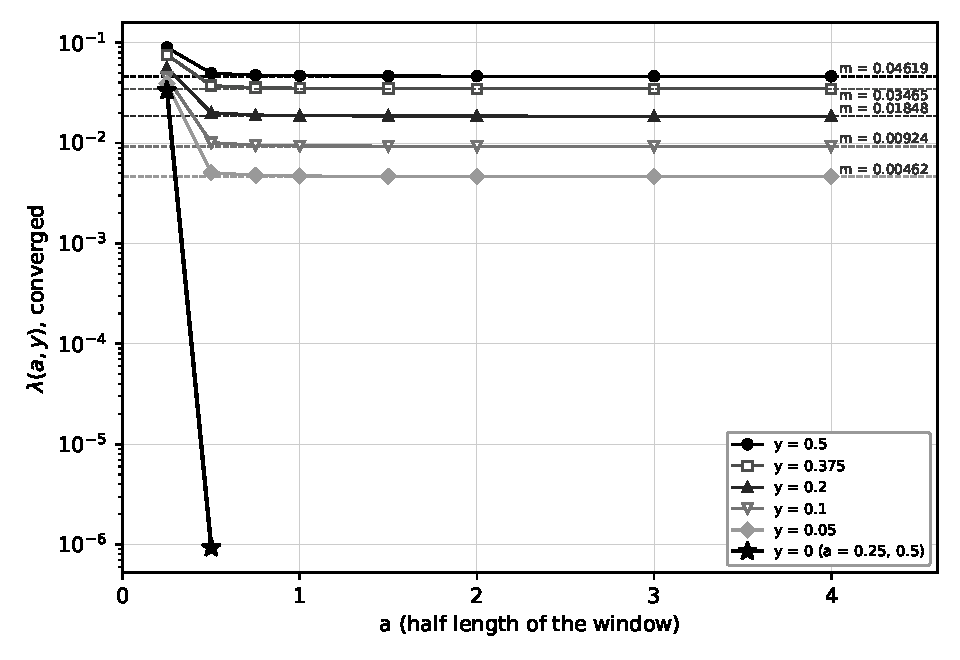
\includegraphics[width=0.9\textwidth]{fig/dc_ladder.pdf}
\caption{The converged ladder on a logarithmic scale: $\lambda_{\min}(\frac12+\varepsilon,a)$ against the window half length $a$ at $a=0.25$, $0.5$, $0.75$, $1$, $1.5$, $2$, $3$, $4$, for $\varepsilon=0.5$, $0.375$, $0.2$, $0.1$, $0.05$ (five marker styles in black and grey), each with the value $2b_{1/2+\varepsilon}$, the limit where the hypotheses of Theorem~\ref{dc:thm:ladder} hold, as a dashed line labelled $m$, and for $\varepsilon=0$ at $a=0.25$ and $0.5$ only (heavy line with stars). The values are those of Table~\ref{dc:tab:ladder}; the legend and the axis write $y$ and $\lambda(a,y)$ for $\varepsilon$ and $\lambda_{\min}(\frac12+\varepsilon,a)$. Drawn by \texttt{code/dc\_ladder.py} (part \texttt{fig}) from \texttt{data/dc\_ladder.json}.}
\label{dc:fig:ladder}
\end{figure}

The decay of the rung at $\varepsilon=0$ is stated four ways in this book: Section~\ref{cp:sec:weil} observes that the least eigenvalue on hat functions falls roughly geometrically in the support length $L=2a$, up to $L=8$; Chapter~\ref{chap:yoshida} observes that the finite sections follow $\exp(-2c\,ae^{2a})$ with $4.1\le c\le5.1$ for $0.25\le a\le0.8$, and does not prove it; Zhu proves, under RH and for large $a$, that the least eigenvalue over real even test functions, and so $\lambda_{\min}(\frac12,a)$, is at most $\exp(-ae^a)$ (Theorem 1.3 of \cite{Zhu26}, Chapter~\ref{chap:zhu}, a preprint); and Theorem~\ref{dc:thm:ladder}(c) proves, under RH, that the rung is $O(a^{-N})$ for every $N$. The four do not conflict: each of these falls is faster than any power of $a$, and Theorem~\ref{dc:thm:ladder}(c) is the weakest of the conditional bounds and the only one whose proof is in the text.

\begin{table}[ht]
\centering\small
\begin{tabular}{@{}cccccc@{}}
\toprule
$\varepsilon$ & $\pi^2v_{1/2+\varepsilon}''(0)/4$ & $a=1$ & $a=2$ & $a=3$ & $a=4$\\
\midrule
$0.5$ & $5.485$ & $6.48$ & $5.92$ & $5.76$ & $5.69$\\
$0.2$ & $2.200$ & $2.68$ & $2.40$ & $2.33$ & $2.29$\\
$0.1$ & $1.100$ & $1.36$ & $1.21$ & $1.17$ & $1.15$\\
\bottomrule
\end{tabular}
\caption{The scaled excess $a^2(\lambda_{\min}(\frac12+\varepsilon,a)-2b_{1/2+\varepsilon})$ in units of $10^{-4}$, against the constant $\pi^2v_{1/2+\varepsilon}''(0)/4$ of Theorem~\ref{dc:thm:ladder}(b): converged $\lambda_{\min}$ (Fourier modes to $1536$, power law extrapolation, as in Table~\ref{dc:tab:ladder}), rounded to three digits. The uncertainty of an entry, the shift of the extrapolation times $a^2$, is at most $4\times10^{-5}$ in these units, an error estimate and not a bound. Script \texttt{code/dc\_rate.py}, parts \texttt{const} and \texttt{table}, data \texttt{data/dc\_rate.json}.}
\label{dc:tab:rate}
\end{table}

The proof of Theorem~\ref{dc:thm:ladder}(b) can be run with numbers, and Table~\ref{dc:tab:bracket} does so (\texttt{dc\_rate.py}, parts \texttt{lower} and \texttt{trial}). Write $\psi(\theta)=v_{1/2+\varepsilon}(\theta)-v_{1/2+\varepsilon}(0)$. The infimum $c_1$ of $\psi(\theta)/\min(\theta^2,1)$ is the limit $v_{1/2+\varepsilon}''(0)/2$ at the origin, on a grid of $600$ points to height $40$ and with the assumption that $\psi$ stays above its minimum on $[20,40]$ beyond $40$, and $\max_\kappa\kappa^2(1-\ell_0(\kappa))=0.5348$ at $\kappa=1.54$, where $\ell_0(1)=0.5726$ and $\ell_0(2)=0.8806$. So the lower constant of the theorem is $c=2c_1\cdot0.5348=0.2167\,\bar c_\varepsilon$ for $a\ge1.54$. Using at every radius at once the bound $P(|\theta|\le r)\le\ell_0(ar)$ for the probability density $|\hat h|^2/\|\hat h\|_2^2$ gives the layer cake bound $\lambda_{\min}-2b_{1/2+\varepsilon}\ge2\int_0^\infty\tilde\psi'(r)\,(1-\ell_0(ar))\,dr$, with $\tilde\psi$ the nondecreasing minorant of $\psi$ in $|\theta|$; it is $0.666\,\bar c_\varepsilon$ at $a=4$, $\varepsilon=\frac12$ ($3.66\times10^{-4}$), and tends to $8I_1/\pi^2\,\bar c_\varepsilon=0.683\,\bar c_\varepsilon$ as $a\to\infty$, with $I_1=\int_0^\infty\kappa\,(1-\ell_0(\kappa))\,d\kappa=0.8425$. These lower bounds are floating point computations on a grid, numerical and not certificates, and for $\varepsilon<\frac12$ the identity $Q_\varepsilon(h)/\|h\|_2^2=2\langle v_{1/2+\varepsilon}\rangle_h$ behind them presupposes that the level is to the right of the zeros.

The cosine trial function of the proof gives upper bounds, computed from the prime side (Table~\ref{dc:tab:bracket}, last column). At $\varepsilon=\frac12$ the ratio of its scaled excess to $\bar c_\varepsilon$ is $1.52$, $1.37$, $1.17$ and $1.11$ at $a=1$, $2$, $4$ and $6$, and $a$ times its remainder over $\bar c_\varepsilon$ is $0.65$ to $0.68$ for $3\le a\le8$, a positive correction of order $a^{-1}$. At $\varepsilon=0.2$ and $0.1$ the remainder oscillates in $a$ ($a$ times it over $\bar c_\varepsilon$ lies between $1.4$ and $2.2$ at $\varepsilon=0.2$ and between $2.3$ and $4.8$ at $\varepsilon=0.1$ for $1.5\le a\le8$), because the tail of $|\hat h|^2$, of order $\cos^2(a\theta)/\theta^4$, meets the peaks of $v_{1/2+\varepsilon}$ at the zeros, of height $1/\varepsilon$, and the cosine is a poor trial function for small $\varepsilon$.

\begin{table}[ht]
\centering\small
\setlength{\tabcolsep}{4pt}
\begin{tabular}{@{}cccccc@{}}
\toprule
$\varepsilon$ & $a$ & lower ($\kappa$) & lower (layer cake) & converged & upper (trial)\\
\midrule
$0.5$ & $1$ & $0.950$ ($1.00$) & $3.834$ & $6.482$ & $8.353$\\
$0.5$ & $2$ & $1.189$ ($1.54$) & $3.692$ & $5.919$ & $7.493$\\
$0.5$ & $4$ & $1.189$ ($1.54$) & $3.656$ & $5.690$ & $6.413$\\
$0.5$ & $6$ & $1.189$ ($1.54$) & $3.661$ & $5.619$ & $6.095$\\
\midrule
$0.2$ & $1$ & $0.381$ ($1.00$) & $1.538$ & $2.678$ & $4.291$\\
$0.2$ & $2$ & $0.477$ ($1.54$) & $1.481$ & $2.401$ & $4.584$\\
$0.2$ & $4$ & $0.477$ ($1.54$) & $1.466$ & $2.295$ & $3.258$\\
$0.2$ & $6$ & $0.477$ ($1.54$) & $1.468$ & $2.262$ & $2.857$\\
\midrule
$0.1$ & $1$ & $0.191$ ($1.00$) & $0.769$ & $1.361$ & $2.813$\\
$0.1$ & $2$ & $0.239$ ($1.54$) & $0.741$ & $1.206$ & $3.745$\\
$0.1$ & $4$ & $0.239$ ($1.54$) & $0.733$ & $1.150$ & $2.331$\\
$0.1$ & $6$ & $0.239$ ($1.54$) & $0.734$ & $1.133$ & $1.863$\\
\bottomrule
\end{tabular}
\caption{Bounds on the scaled excess $a^2(\lambda_{\min}(\frac12+\varepsilon,a)-2b_{1/2+\varepsilon})$, in units of $10^{-4}$: the lower bound of the proof of Theorem~\ref{dc:thm:ladder}(b) with the single radius $\kappa\le a$ that maximises $\kappa^2(1-\ell_0(\kappa))$ (the radius in brackets), the layer cake lower bound, the converged value (as in Table~\ref{dc:tab:rate}, extended to $a=6$ in \texttt{data/dc\_rate.json}), and the value of the trial function $\cos(\pi u/2a)$ computed from the prime side, which is an upper bound. Script \texttt{code/dc\_rate.py}, parts \texttt{lower} and \texttt{trial}.}
\label{dc:tab:bracket}
\end{table}
